\scanpage{21}
\figure{
\begin{tikzpicture}[x=1mm,y=1mm]
\fill[gray] (-20.2,1.65) circle (.1);
\fill (-4.3,-.55) circle (.18);
\draw[gray,very thin] (-4.1,-.48)--(-.7,-.08);
\fill (0,0)--(.4,.65)--(2.8,1.55)--(5.65,2)--(6.3,1)--(7.1,.35)--(6.3,.2)--(4.8,.5)--cycle;
\end{tikzpicture}}

\begin{center}Prof Grothendieck\hspace{1.6em}\unsure{.}\end{center}

\figure{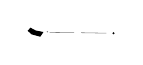
\begin{tikzpicture}[x=1mm,y=1mm]
\fill (0,.4)--(.35,.8)--(1,.45)--(2,.25)--(1.6,-.35)--(.5,-.05)--cycle;
\draw[gray,very thin] (2.8,.2)--(5.9,.16) (6.8,.16)--(10,.1);
\fill[gray] (2.5,.29) circle (.09);
\fill (10.9,.1) circle (.15);
\end{tikzpicture}}

\figure{\begin{tikzpicture}[x=1mm,y=1mm]
\draw[gray,very thin] (.2,.9) to[bend right=35] (.2,0);
\fill (10.9,.8)--(11.3,1.2)--(12,.9)--(11.85,.5)--(11,.55)--cycle;
\end{tikzpicture}}
% archive sheet number: 20.
\clearpage
